\subsection{Datomic}
\label{datomic}

Datomic \cite{datomic} is another project started by Rich Hickey and is now
developed and marketed by \textit{Cognitect Inc} besides Clojure, a Lisp
dialect for the JVM, originally conceived by Hickey, as was introduced in
chapter \ref{LanguageOfTheSystem}.

Instead of being another functional programming language, Datomic
is a distributed data base, delivering classic data base guarantees and
features like ACID transactions, joins and a logical query language.
The main difference however, is that Datomic is based on the
value-oriented idea of immutable data and not based on the idea of
mutable cells in a table (as demonstrated by Fig.\ref{sql} in
chapter \ref{LanguageOfTheSystem}) as explained in
\cite{datomic-architecture} and \cite{datomic-datamodel}.
This is why one of Hickey's talks about Datomic \cite{datomic-talk1},
\cite{datomic-talk2} is called \textit{The Database as a Value}.

As introduced in chapter \ref{LanguageOfTheSystem} Hickey views
data values as facts. Therefor a data base's role of storing data
is nothing more than the accretion of facts, in the same way
that history is an accretion of facts, like ``the king died'' or
``Today I moved to Berlin.'' and even though new facts can be
recorded concerning the same subject or \textit{entity}, these
new facts do \textit{not} invalidate that there was a point in time
in which the old fact was true. New facts do not overwrite old facts.

\begin{figure}[h]
  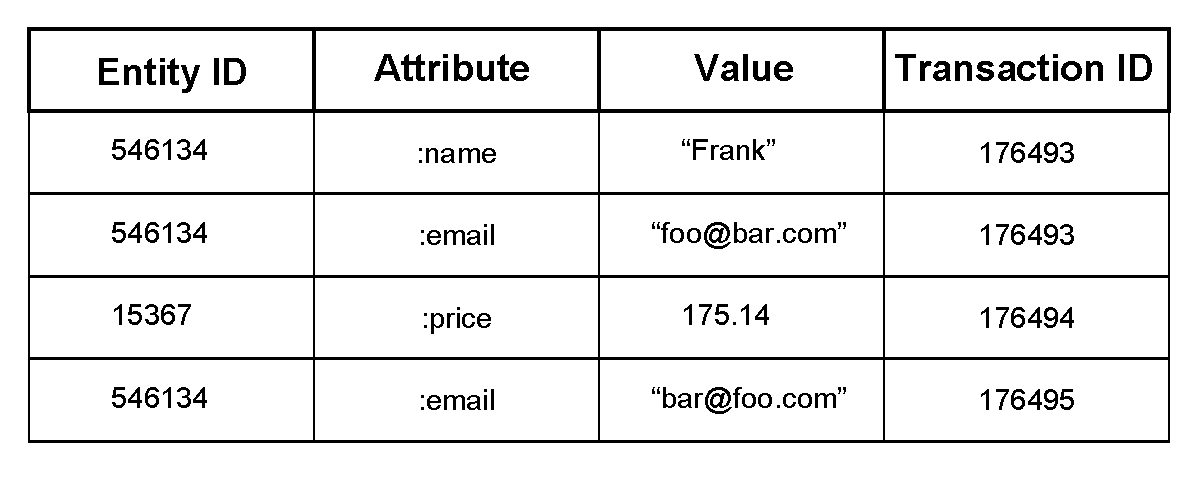
\includegraphics[scale=0.6, keepaspectratio]{datomic_scheme.pdf}
  \caption{The information model schema used in Datomic.}
  \label{datomic_schema}
\end{figure}

So in order to talk about facts at different points in time, Datomic
uses a single schema information model which defines the structure
of every recorded fact. As shown in Fig.\ref{datomic_schema} every
fact is a 4-tuple consisting of an entity ID to uniquely identify
subject for which a new fact is recorded for, the attribute of
the entity for which this is new information, the actual value itself
that we want to record and a transaction ID that serves as a logical
time stamp in order to allow facts to be recorded at different points
in time. The idea of logical time is of course in reference to what is
known as a \textit{Lamport Clock} \cite{lamportclock} and also
\textit{Vector Clocks} \cite{vectorclock1}, \cite{vectorclock2}
and has been used by other distributed storage systems like
Google's \textit{Bigtable} project \cite{bigtable}.

In contrast to the example shown in Fig.\ref{sql} in
chapter \ref{LanguageOfTheSystem} the example shown here in
Fig.\ref{datomic_schema} tries to show how a possible snapshot of
the distributed log of facts might look like in Datomic. As one
can see the first transaction (\#176493) sets two attributes of
the same entity, namely its name and email address. The next
transaction sets the price of some completely different entity
and then another transaction is issued concerning the already
existing entity from the first transaction, recording a new email
address for that entity.

This of course means, that any reader still reading the old
email address won't be interrupted and can still perceive his
outdated view of the world and any new reader can decide whether
he wants to receive the most recent value or the history of a
value. This lends itself to using timed window operations in order
to select only a fraction of the history and brings this system
closer to the field of data streams and event stream processing.



